\documentclass[fleqn,a4paper,12pt]{article}
\usepackage[top=1in, bottom=1in, left=1in, right=1in]{geometry}



\title{Machine Learning Homework 4}
\date{}

\setcounter{section}{2}

\usepackage{listings}

\usepackage{amsmath}
\usepackage{amssymb}


\usepackage{mathspec}
\setmainfont{Noto Serif CJK TC}
% \setmathsfont(Digits,Latin,Greek)[Numbers={Lining,Proportional}]{DejaVu Math TeX Gyre}
\newfontfamily\ZhFont{Noto Serif CJK TC}
\newfontfamily\SmallFont[Scale=0.8]{Droid Sans}
% \newfontfamily\SmallSmallFont[Scale=0.7]{Noto Serif CJK}
\usepackage{fancyhdr}
\usepackage{lastpage}
\pagestyle{fancy}
\fancyhf{}
\rhead{B03902072\ZhFont{江廷睿}}
\lhead{Machine Learning Homework 4}
\rfoot{\thepage / \pageref{LastPage}}

\XeTeXlinebreaklocale "zh"
\XeTeXlinebreakskip = 0pt plus 1pt
\usepackage{parskip}

\usepackage{graphicx}
\usepackage{caption}
\usepackage{subcaption}
\usepackage{float}

\begin{document}
% \maketitle
\thispagestyle{fancy}

\subsection*{1.1. Dataset 中前 10 個人的前 10 張照片的平均臉和 PCA 得到的前 9 個 eigenfaces}

\begin{figure}[H]
\centering
\begin{subfigure}{.1\textwidth}
  \centering
  
\includegraphics[width=\linewidth]{problem1/avg-face.png}
  \caption{平均的臉}
  \label{fig:sub1}
\end{subfigure}%
\begin{subfigure}{.3\textwidth}
  \centering
  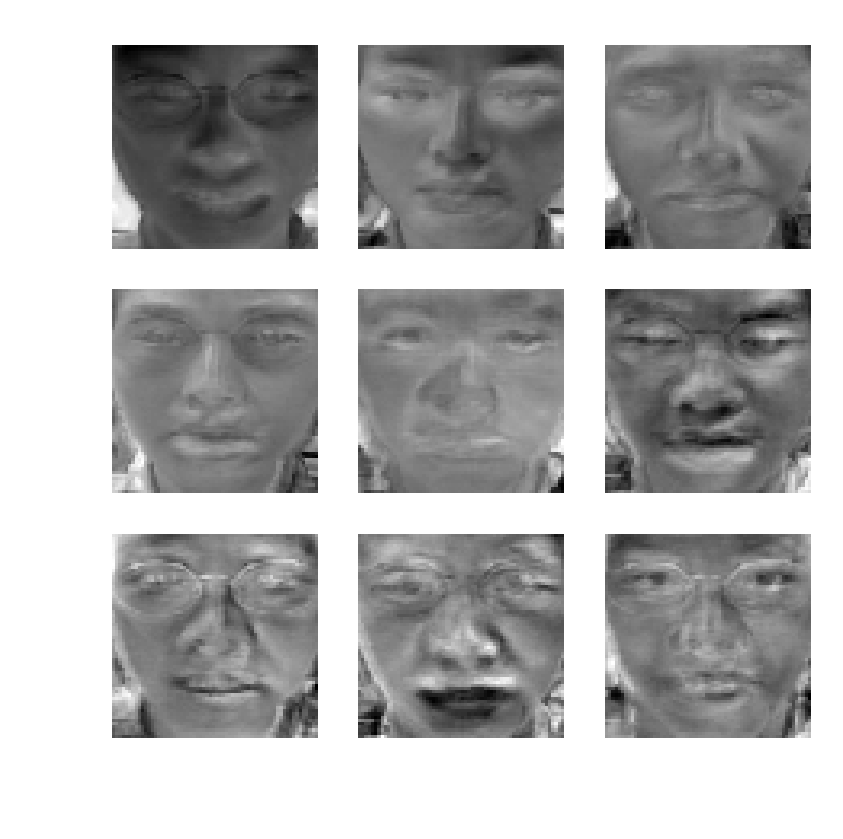
\includegraphics[width=\linewidth]{problem1/eigen-faces.png}
  \caption{特徵臉}
  \label{fig:sub2}
\end{subfigure}
% \caption{1.1}
\label{fig:p1.1}
\end{figure}

\subsection*{1.2. Dataset 中前 10 個人的前 10 張照片的原始圖片和 reconstruct 圖 (用前 5 個 eigenfaces)}

\begin{figure}[H]
\centering
\begin{subfigure}{.5\textwidth}
  \centering
  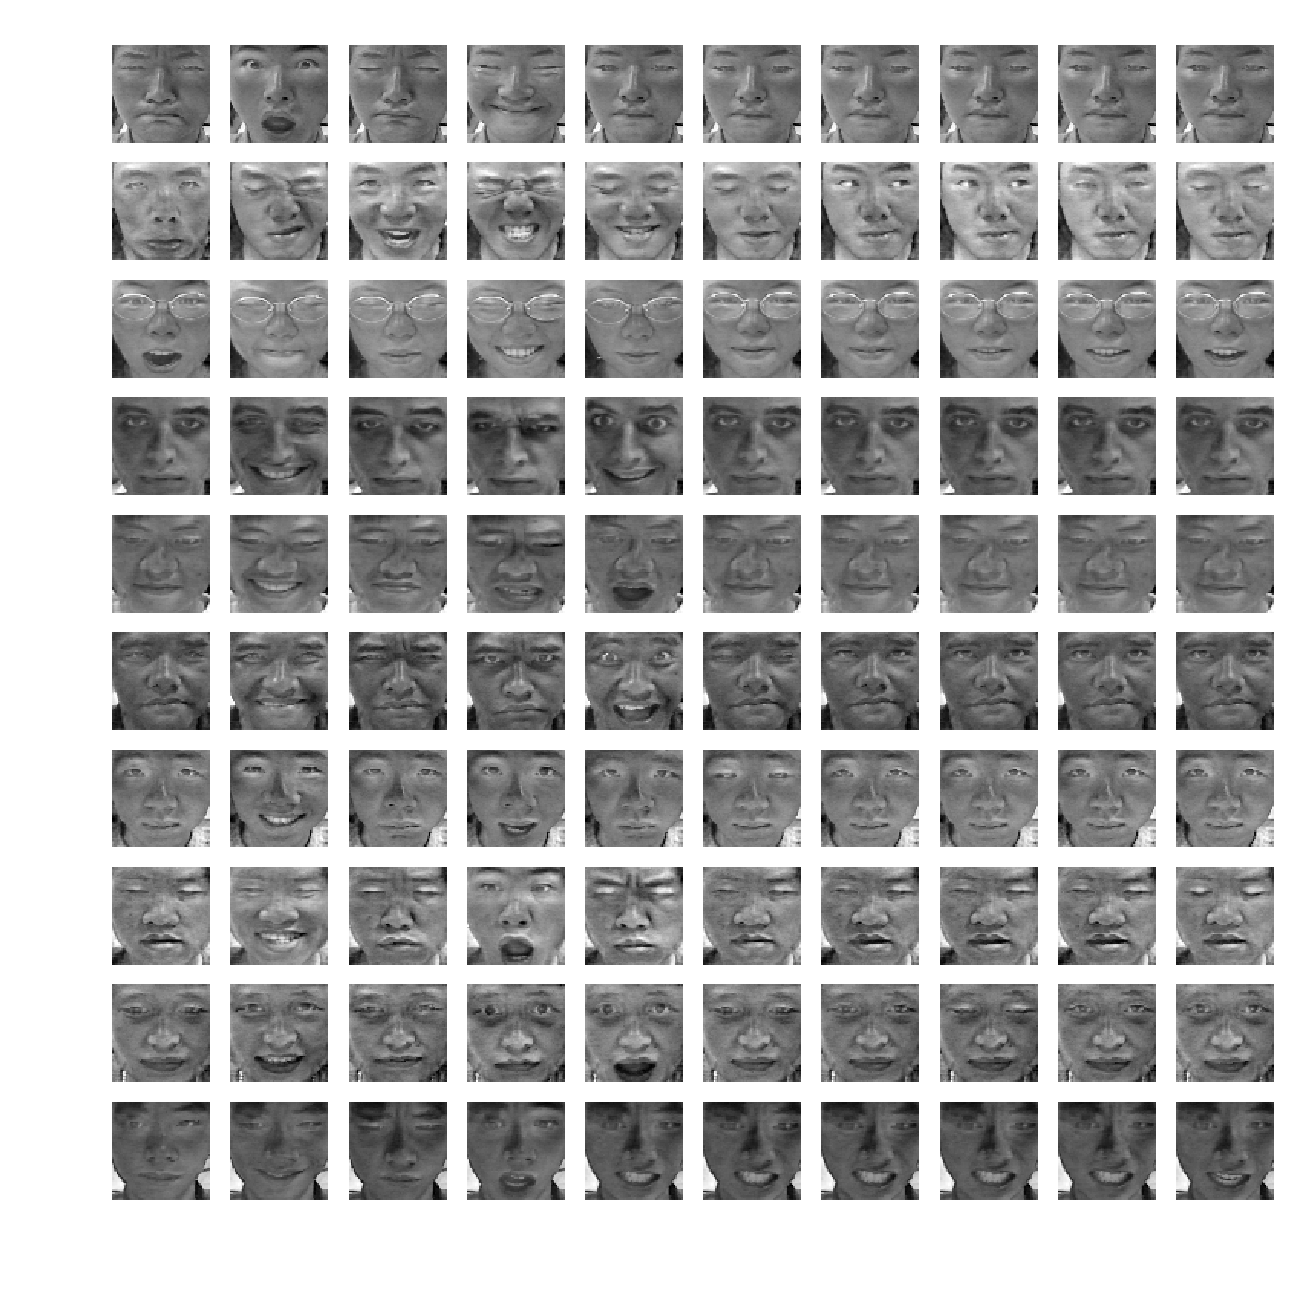
\includegraphics[width=\linewidth]{problem1/orig-faces.png}
  \caption{原來的臉}
  \label{fig:sub1}
\end{subfigure}%
\begin{subfigure}{.5\textwidth}
  \centering
  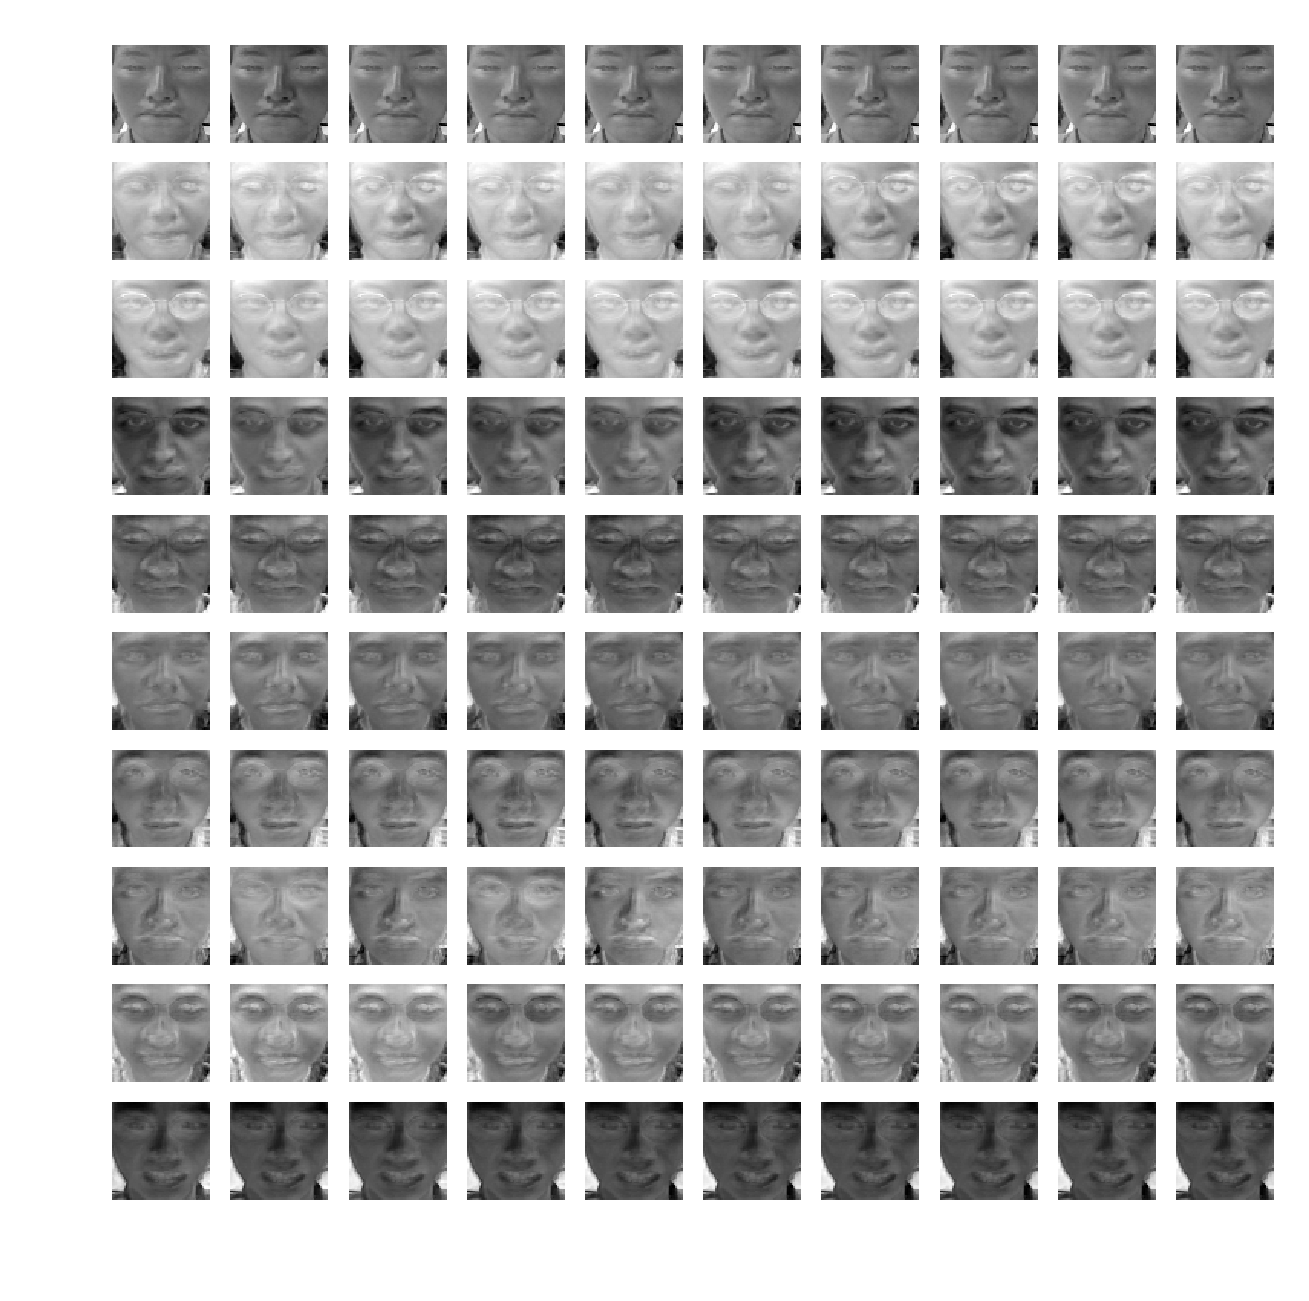
\includegraphics[width=\linewidth]{problem1/projected-faces.png}
  \caption{重建後的臉}
  \label{fig:sub2}
\end{subfigure}
% \caption{1.1}
\label{fig:p1.1}
\end{figure}


\subsection*{1.3. Dataset 中前 10 個人的前 10 張照片投影到 top k eigenfaces 時就可以達到 < 1\% 的 reconstruction error}

$k = 59$

\subsection*{2.1. 使用 word2vec toolkit 的各個參數的值與其意義}

\begin{itemize}
\item \textbf{size}: 最後訓練出來的詞向量的維度。使用預設值 100 。
\item \textbf{window}: 訓練詞向量時,要考慮的前後詞彙的總數量加一。使用預設值 5 。
\item \textbf{sample}: 減少取樣出現頻率大於這個參數的詞彙,以加快訓練速度。使用預設值 1e-3 。(雖然註解說預設值是 0 ,但原始碼裡預設是 1e-3 )
\item \textbf{hs}: 是否使用階層化的 softmax ,藉由樹狀的結構,先預測較大的類別再從該類別預測較小的類別,如此一來勳練時每次都只需要更新從根到正確預測所經過的節點,可以大幅增快訓練速度。使用預設值 1 。
\item \textbf{negative}: 在訓練時,那些被取樣以更新相關權重的錯誤詞彙數量。較大的取樣數量可能會增加詞向量的品質,但會減慢訓練速度。使用預設值 5 。
\item \textbf{min\_count}: 忽略出現次數少於此數量的詞彙。使用預設值 5 。
\item \textbf{alpha}: 起始學習率。
\item \textbf{cbow}: 是否使用 CBOW 的方式(0)或是 skip gram 的方式(1)訓練。使用預設值 1 。CBOW 的方式是從前後文預測中間的詞彙,而 skip gram 則是從中間的詞彙預測前後文。
\end{itemize}

\subsection*{2.2. 將 word2vec 的結果投影到 2 維的圖}

\begin{figure}[H]
\centering
\includegraphics[width=0.8\linewidth]{tsne-cropped.png}
\caption{使用 tSNE 投影}
\label{fig:p2.2}
\end{figure}


\subsection*{2.3. 從上題視覺化的圖中觀察到了什麼?}

大致來說,除了 NN 以外,詞性相同的詞彙會聚集成幾個分開小群。但因為詞向量的訓練方式,主要考量的可能會是詞會的語意,所以相同詞彙的詞並沒有聚集成單一個大群。同時,詞性為 NN 的詞彙可能也是因為這些詞彙包含太多語意,或是因為它們佔訓練資料的大多數,所以較為平均的散佈在二維的空間中。

\subsection*{3.1. 請詳加解釋你估計原始維度的原理、合理性,這方法的通用性如何?}

\par
\textbf{方法}:對於所有 $d \in [1, 60]$,使用助教生成資料的程式碼生成隱含維度為 $d$ 維資料,再從生成出來的資料中隨機抽取 100 個點,算出它們與最近的點的平均距離。重複 20 次後得到 20 個平均距離,計算這 20 個平均距離的平均數與標準差,發現隨著隱含維度 $d$ 的上升,平均距離亦有上升的趨勢,且標準差皆相對不大。尤其對於低隱含維度的資料,標準差遠小於相鄰隱含維度之距離平均之差。因此可以對於每筆測試資料,同樣取樣 100 個點並計算最近點距離的平均,並與用前面說的方法所得到每一維度的平均距離比較,取平均最相近的維度作為預測結果。

\textbf{原理}:猜測是因為當隱含維度愈高時,資料點在原來空間的分佈會愈稀疏,因此在轉換到高維後資料點的距離也會稀疏。

\textbf{合理性}:因為對於同一維度的資料,觀察到的平均最近點距離標準差不高,且統計的資料與測試的資料遵循相同的分佈,因此十分合理。

\textbf{通用性}:通用性不高,因為對於一般的資料,我們無從統計其原始隱含維度與最近點的平均距離,且不同資料從低維轉換到高維的過程也不一致,也不一定具有相同的性質,因此此方法只適用於此作業。

\subsection*{3.2. 將你的方法做在 hand rotation sequence datatset 上得到什麼結果?合理嗎?請討論之。}

結果得到 4 。此資料集的實際隱含維度估計應該是 3 ,因為該序列幾本上可以算是視角的是水平旋轉,因此所有圖片的集合可以對應到一個圓柱表面的座標系統,而其維度是 2;而每張圖片都對應到此圓柱表面的一個角度,所以總維度會是 2 + 1 。雖然 4 / 3 相對來說有點高,但相減的誤差而言,應該算是還可以接受。這也代表了此方法也許比想像中的通用一些。


\end{document}
